\documentclass[a4paper,12pt]{article}
\usepackage[lmargin=1cm,rmargin=1cm,tmargin=1cm,bmargin=1.5cm]{geometry}
 % \usepackage[utf-8]{inputenc} (si lo pones tienes problemas y la verdad no se por que . 
\usepackage[spanish]{babel}%para que te aparezca capitulo 1 en vez de chapter 1
\usepackage{amsmath}
\usepackage{amsfonts}
\usepackage{amssymb}
\usepackage{float} % Este sive para usa el [H] en el begin figure
\parindent=0mm %con esto elimino la sangría 
\usepackage{graphicx}
\usepackage{caption} % Necesario para poner caption
\usepackage{subcaption} % Necesario para las subfiguras 

\usepackage{circuitikz} %este es el paquete para crear circuitos electricos 
\usepackage{siunitx} %este paquete es para las unidades de medida

\newtheorem{preg}{Pregunta} %este es para las preguntas 

\usepackage{enumitem} % Este me sive para modificar el description , itemize y otros 


\begin{document}

\begin{itemize}
\item Nombre : Juan Alonso Alcalá Lujan 
\item Código : 20172226A 
\end{itemize}

% PREGUNTA NUMERO 1 
\begin{preg}
Establezca las ecuaciones del circuito puente de wheastone de la figura. 
\begin{itemize}
 \item a) Analice las mallas, establezca las ecuaciones para determinar las corrientes en cada resistencia ¿Cómo se determinaría el valor de la corriente $I_5$ en la resistencia $R_5$ ?  
 
 \item b) Determine la condición de balance del puente.
\end{itemize} 
\end{preg}

\begin{figure}[H]
\begin{center}
\begin{circuitikz}[american]
\draw (0,0)  to[battery,a= V,*-*] (0,4) node[label={above:f}]{}
             to[] (4,4) node[label={above:a}]{} to[R , a=$R_1$, *-*,f>_=$i_1$] (2,2) node[label={left:b}]{} to [R , a=$R_3$,*-*,f>_=$i_1-i_5$] (4,0) node[label={below:d}]{} ;
\draw (0,0) node[label={below:e}]{} to [] (4,0) to[R,a=$R_4$,f<_=$i_5+i_2$] (6,2) node[label={right:c}]{} to [R,a=$R_2$,*-,f<_=$i_2$] (4,4) ;

\draw (2,2) to[R,a=$R_5$,f=$i_5$] (6,2);

\end{circuitikz} 
\end{center}
\caption{Puente de Wheatstone}
\end{figure}

Aplicando la 2da ley de kirchoff en las mallas abc , bdc y efd obtenemos las siguientes 3 ecuaciones . 
\begin{align*}
R_{1} i_{1} - R_{2} i_{2} + R_{5} i_{5} &= 0 \\
R_{3} i_{1} - R_{4} i_{2} + i_{5} \left(- R_{3} - R_{4} - R_{5}\right) &= 0 \\
- R_{3} i_{5} + i_{1} \left(R_{1} + R_{3}\right) &= V 
\end{align*}

En forma matricial : 

$$
\left[\begin{matrix}R_{1} & - R_{2} & R_{5}\\R_{3} & - R_{4} & - R_{3} - R_{4} - R_{5}\\R_{1} + R_{3} & 0 & - R_{3}\end{matrix}\right]\left[\begin{matrix}i_{1}\\i_{2}\\i_{5}\end{matrix}\right] =  \left[\begin{matrix}0\\0\\V\end{matrix}\right]
$$

De esta manera hallamos las intensidades en cada resistencia . Como ejemplo hallemos $i_5$ usando regla de Cramer

$$
i_5 = \dfrac{\left|\begin{matrix}R_{1} & - R_{2} & 0\\R_{3} & - R_{4} & 0\\R_{1} + R_{3} & 0 & V\end{matrix}\right|}{\left|\begin{matrix}R_{1} & - R_{2} & R_{5}\\R_{3} & - R_{4} & - R_{3} - R_{4} - R_{5}\\R_{1} + R_{3} & 0 & - R_{3}\end{matrix}\right|}
$$ 
Cuya respuesta es : 
$$
i_5 = \frac{- R_{1} R_{4} V + R_{2} R_{3} V}{R_{1} R_{3} R_{4} - R_{2} R_{3}^{2} - R_{2} \left(R_{1} + R_{3}\right) \left(- R_{3} - R_{4} - R_{5}\right) + R_{4} R_{5} \left(R_{1} + R_{3}\right)}
$$

De acá es fácil ver que la condición del balance de puente es :
$$
R_{1} R_{4}  = R_{2} R_{3}
$$

\begin{preg}
¿Que es un sensor ? Indique los tipos de sensores
\end{preg}

Un sensor es todo aquello que tiene una propiedad sensible a una magnitud del medio, y al variar esta magnitud también varia con cierta intensidad la propiedad, es decir, manifiesta la presencia de dicha magnitud, y también su medida.\\

\textbf{Tipos}



\begin{itemize}
\item De contacto, proximidad
\item Ópticos (De color, luz)
\item De sonido
\item Térmicos
\item De humedad
\item Magnéticos
\item De infrarrojos
\end{itemize}




\begin{preg}
Investigar el principio físico, curvas características o funciones que relacionen las variables físicas, materiales de fabricación, tiempo de respuesta y limitaciones de uso de :
\begin{itemize}
\item a) Un termistor(indicar el significado de su coeficiente de temperatura)
\item b) Una fotorresistencia
\end{itemize}
\end{preg}


\begin{itemize}

\item \textbf{\large{Termistor}}
\begin{description}[leftmargin=0.2cm]
\item[Principio Fisico:] El funcionamiento se basa en la variación de la resistencia de un semiconductor debido a cambios en la temperatura ambiente, alterando la concentración de portadores dentro de el .

\item[Relación entre variables Físicas] Existen dos tipos de termistores . NTC ( las de coeficiente de temperatura negativo ) y PTC ( las de coeficiente de temperatura positivo ) Sus gráficos se muestran a continuación . 

\begin{figure}[H]
\centering
 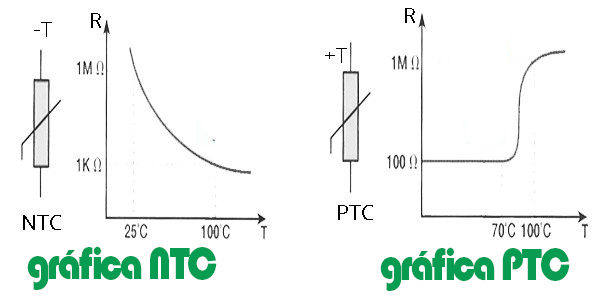
\includegraphics[width=0.5\textwidth]{NTCandPTC.jpg}
  \caption{Relación entre La Temperatura y la Resistencia del elemento . El primero es una relacion negativa y el segundo una relación positiva}

\end{figure}


\item[Materiales de Fabricación:] Se fabrican a partir de los óxidos de metales de transición (manganeso, cobalto, cobre y níquel). El silicio y germanio también se utilizan en la fabricación de termistores.

\item[Coeficientes de resistencia de Temperatura ($\alpha$):] Se define a una temperatura "T'' como  
$$ \alpha_{T} = \dfrac{1}{R_{(T)}}\dfrac{dR_T}{dT} $$
Es una propiedad intensiva de los termistores e indica cuan rápido cambiara el valor de la resistencia del elemento en las proximidades de un valor de Temperatura . 
\end{description}

\item \textbf{\large{Fotorresistencia}}

\begin{description}[leftmargin=0.2cm]
\item[Principio Fisico:] Se basa en el fenómeno del efecto fotoeléctrico 

\item[Relación entre variables Físicas] En la siguiente gráfica se ve la relación entre la Intensidad de incidencia de luz y la resistencia . 

\begin{figure}[H]
\centering
 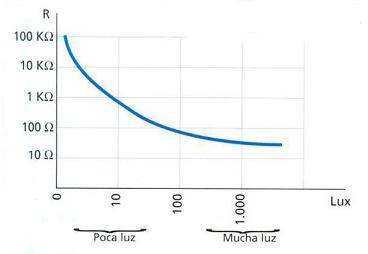
\includegraphics[width=0.5\textwidth]{fotoresistor.jpg}
  \caption{Intensidad vs Resistencia}

\end{figure}


\item[Materiales de Fabricación:] Un fotorresistor está hecho de un semiconductor de alta resistencia como el sulfuro de cadmio , sulfuro de plomo y seleniuro de cadmio .

\item[Tiempo de respuesta:] típico está en el orden de una décima de segundo.
\end{description}



\end{itemize}




\begin{preg}
Diferencie la resistividad $\rho$ de (a) un conductor (b) un semiconductor (c) ¿Cómo varia $\rho$ con la temperatura en cada caso ? 
\end{preg}



\begin{itemize}
\item Un \textbf{conductor}  tal como un metal tiene alta conductividad y por tanto baja resistividad mientras que un \textbf{semiconductor} su conductividad esta entre la de un conductor y un aislante . El superconductor varia ampliamente en diferentes condiciones (ej exposición de campo eléctrico o frecuencias especificas de la luz y la composición del material ) . 

\item \textbf{Dependencia de la resistividad con la temperatura (caso conductor)}. La resistividad de los conductores aumenta con el aumento de la temperatura. A medida que aumenta la temperatura del conductor, aumenta la velocidad promedio de los electrones que son los portadores de corriente. Como resultado aumenta el número de colisiones y el tiempo promedio de colisiones disminuye con la temperatura. Dado que la resistividad es inversamente proporcional al tiempo promedio ,entonces, la resistividad aumenta


\item \textbf{ Dependencia de la resistividad con la temperatura en el conductor}.
En semiconductores, la resistividad disminuye con el aumento de la temperatura. A medida que aumenta la temperatura, el número de portadores de carga aumenta debido a la ruptura de más y más enlaces covalentes. Por lo tanto, su conductividad aumenta y la resistividad disminuye con el aumento de la temperatura.


\end{itemize}


\end{document}
